% !Mode:: "TeX:UTF-8"
%% 请使用 XeLaTeX 编译本文. 默认使用 Adobe 字体. 需自行安装.
%%文件名不能出现任何中文字,否则反向查询功能不能实现
\documentclass{mytemplate}% 选项 forprint: 交付打印时添加, 避免彩色链接字迹打印偏淡. 即使用下一行:
%\documentclass[forprint]{mytemplate}
\usepackage{abstract,float}
\usepackage{makecell}
\setmainfont{Times New Roman}

%%===参考文献===%%%%%%%%%%%%%%%%%%%%%%%%%%%%%%%%
\bibliographystyle{abbrv}        % 参考文献样式,  plain,unsrt,alpha,abbrv,chinesebst 等等
%%%%%%%%%%%%%%%%%%%%%%%%%%%%%%%%%%%%%%%%%%%
\graphicspath{{figures/}}        % 图片文件路径
%%%%%%%%%%%%%%%%%%%%%%%%%%%%%%%%%%%%%%%%%%%
\allowdisplaybreaks
%%%%%%%%%%%%%%%%%%%%%%%%%%%%%%%%%%%%%%%%%%%
%\setmainfont{Times New Roman}
\begin{document}
%%%%%%% 下面的内容, 据实填空.
\baselineskip=14pt  % 正文行距为 20 磅
\setlength{\columnsep}{22pt}

%----------------------------------------------------------------------------

\renewcommand{\thefootnote}{\fnsymbol{footnote}}
%\mytitle
%\simpletitle

%\coverpage

%\frontmatter
%\newpage
%\pagenumbering{arabic}%Roman  % 正文之前的页码用大写罗马字母(Roman)编号.也可选用arabic (阿拉伯数字)
%%-----------------------------------------------------------------------------
%\include{includefile/frontmatter}    % 加入摘要, 申明.
%==========================把目录加入到书签==============================%%%%%%
%\pdfbookmark[0]{目录}{toc}

\vspace{0.5cm}

\begin{flushleft}
{\zihao{-4} \heiti Final Report}
\end{flushleft}
\vspace{1cm}
\begin{center}
{\zihao{4}  \textbf{Marketing Campaign Candidate Analysis}}\\
\vspace{0.2cm}
{\zihao{5}Yiheng Xiao (yx426), Chen Zhong (cz379)}
\end{center}
\vspace{0.5cm}
\begin{enabstract}
 Successful market Campaign boosts business by promoting products effectively. The important question here is how to choose the pool of potential customers to increase success rate. Our project is to propose a data mining approach to classify the best set of clients using contact records and clients' features. All Codes are in {\color{green}\texttt{"midterm.ipynb"}}.
\end{enabstract}
\vspace*{2em}
%%%%%%%%%%%%%%%%%%%%%%%%%%%%--------main matter-------%%%%%%%%%%%%%%%%%%%%%%%%%%%%%%%%%%%%

\setcounter{page}{1}
\setlength\parindent{0em}
\columnsep=20pt
\begin{multicols}{2}
\tableofcontents
\section{\color{blue} Project Introduction}
Marketing campaign is essential for any business in any industry to grow customers and expand business. A successful company requires not only good product but also a good way to advertise its product. One of the most traditional yet effective way of marketing campaign is through phone calls. These phone-call based marketing campaigns are done by making phone calls to a pool of potential customers to promote certain products. Unfortunately, in order to increase the rate of success many potential customers will be called more than once. While it takes a lot of time and effort to attract a new customer, very often people will feel uncomfortable about the repetitive phone calls and may even jeopardize the campaigning company’s reputation.

The important question here is how to choose the pool of potential customer to increase success rate? If we can increase
success rate of phone call marketing campaigns, less resource is required to attract each new customer and it is less likely
to have negative advertising effect.

Our approach to the problem is to analyze market campaign data, which includes information about the background of customers and try to determine the specific profile of customers who will be more likely to subscribe the product in campaign. More specifically, our project is to propose a data mining approach to select the best set of clients that are more likely to subscribe a product through tele-marketing calls.

\section{\color{blue}Initial Processing and Visualization}
\subsection{Raw Data}
We selected the Bank Marketing Data Set\footnote{http://archive.ics.uci.edu/ml/datasets/Bank+Marketing} from UCI Machine Learning repository. The data is taken from the direct marketing campaigns of a Portuguese banking institution. The marketing campaigns were based on phone calls. The data set consists of a list of 45211 samples with 20 features. We are interested in whether we can predict the "y" feature, which is the whether the particular sample subscribed to the product or not, using all other features given about that particular sample. Below is a list of sample important features {\color{red}Table \ref{t01}}.
\begin{table}[H]
  \centering
  \begin{tabular}{|l|l|l|}
     \hline
Client data & Description&Type \\ \hline
age & age of clients &numeric\\ \hline
 job & type of job&categorical\\ \hline
 marital & marital status&categorical\\ \hline
 education & level of education& categorical\\ \hline
 default & whether has credit in default& categorical\\ \hline
 housing & whether has housing loan& categorical\\ \hline
 loan  &whether has personal loan& categorical \\ \hline
   \end{tabular}
  \caption{Several Features}\label{t01}
\end{table}

\subsection{Initial Data Cleaning}
First thing we looked at was missing values. Besides the "poutcome" feature, most other features have similar amount of samples, to allow for initial steps, we filled the n/a values in "poutcome" and "default" with string "nonexistent" and proceeded to exclude all other n/a's, which result in a clean set of data with 38245 samples (The majority of samples (85\%)  are included, the method of dealing with missing value is acceptable) . We will try to preserve more data in the future.

Since we are dealing with many categorical and binary attributes, we used one hot encoding for categorical features (each category as a new feature and has binary value), and we transformed binary attributes to {0,1}. Which expands the data set to having 54 features. Reason for one-hot-encoding is that regression analysis requires numerical values, and each category as a feature allows our models to compare the affect of each category independently and makes it easier for us to eliminate some of the features.

\subsection{Visualization}
\subsubsection{General}
%![plot](https://github.com/Johnzhong1468/MarketingCampaign/blob/master/3d_age_dur_pd.PNG)<br>
\begin{figure}[H]
  \centering
  % Requires \usepackage{graphicx}
  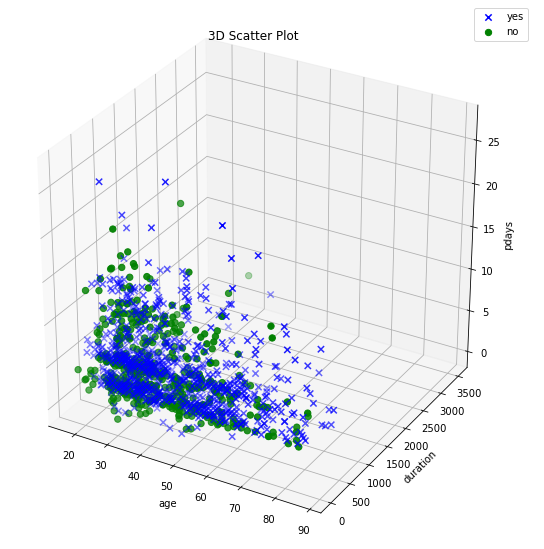
\includegraphics[width=7.5cm]{3d_age_dur_pd.PNG}\\
  \caption{Visualization 1}\label{g01}
\end{figure}

To First try to understand the data, we want to explore the relationship between some of the important features (see {\color{red}Graph \ref{g01}}), here we chose age, duration of previous contact(duration), and number of days past after previous contact(pday). We also restricted the data to people who have been contacted more than once. People who accepted the product are color coded with blue and those who didn't are green. We can see that there are a lot of people that actually accepted the product under the condition that they were contacted more than once. We can see that more samples have low duration and small pdays, and more samples are in the young age group than old age group. However for determining whether a sample accept the product, age does not seem to have a big effect graphically since "yes" samples have a similar profile as "no" sample. However duration and pday seem to have distinct affect, and we will explore that further in the future.
\begin{figure}[H]
  \centering
  % Requires \usepackage{graphicx}
  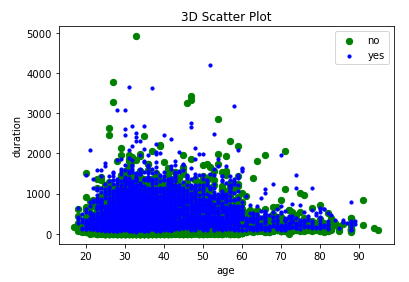
\includegraphics[width=7cm]{age_dur_scatter.PNG}\\
  \caption{Visualization 2}\label{g02}
\end{figure}

This plot shows the group of people who were only contacted once. We can see again that age has the same distribution profile among the "yes" and "no" group.
\begin{figure}[H]
  \centering
  % Requires \usepackage{graphicx}
  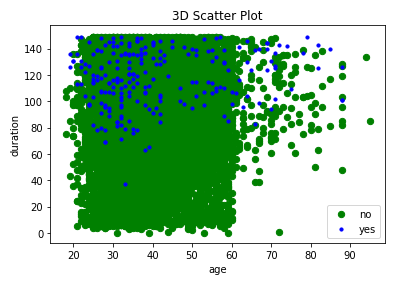
\includegraphics[width=7cm]{age_dur_scat_shrt.PNG}\\
  \caption{Visualization 3}\label{g03}
\end{figure}

%![plot](https://github.com/Johnzhong1468/MarketingCampaign/blob/master/age_dur_scat_shrt.PNG)<br>
We shrink duration to less than 150 and as expected people are likely to reject when the duration of the call is very short.
\subsubsection{Correlation Visualization}
\begin{figure}[H]
  \centering
  % Requires \usepackage{graphicx}
  \includegraphics[width=7cm]{corr.png}\\
  \caption{Correlation}\label{g04}
\end{figure}

Data visualization is a very useful tool to better
explore which variables are important in
determining the house price. Firstly, a correlation graph is plotted
to visualize which variables could influence the "y" (subscribe our service or not) distinctively and get better sense of the correlations.

As we can see from Figure \ref{g04}, the variables are of low linear correlation. Variables such as "(Connection) Duration", "(previous) days" are highly correlated with our target "y".

\section{\color{blue}Model Selections}
\subsection{General Procedures}
The project focuses on a classification problem, so, we set a hypothesis set H including linear models with regularizer, Logistic regression models, Supporting Vectors Machine as well as Decision trees. To find the model with satisfying explanatory ability, the model selection obeys the following procedures:

\begin{enumerate}
  \item ~~Fit models in training set, remove non-significant features.
  \item ~~Select the optimal hyper-parameters by cross validation.
  \item ~~Compare the Prediction Accuracy computed on traning set and testing set.
  \item ~~Analyze results of different models.
\end{enumerate}
\subsection{Quadratic Loss}
The intuition in using a linear model with quadratic
loss is straightforward. The explanatory variables are most likely to have a linear relationship with "y". The objective function of this linear model is defined as 

\begin{equation}
\min \sum_{i=1}^n(y_i-w^Tx_i)^2+r(w)
\end{equation}
\subsubsection{Quadratic Loss with $l_1$ Regularization( Lasso Model)}
Lasso regression performs covariate selection as well as improves prediction error by shrinking large regression coefficients in order to reduce overfitting. However, it may not effective in solving classification problems; the accuracy of Lasso is merely 2.10\%, which fails to meet our expectation. From {\color{red} graph \ref{g05}}, the predicted value is highly biased. 
\begin{equation}\label{eq01}
  \min \sum_{i=1}^n(y_i-w^Tx_i)^2+\lambda\sum_{i=1}^n|w_i|
\end{equation}

\begin{figure}[H]
  \centering
  % Requires \usepackage{graphicx}
  \includegraphics[width=6cm]{lasso.png}\\
  \caption{lasso}\label{g05}
\end{figure}

\subsubsection{Quadratic Loss with $l_2$ Regularizer (Ridge)}
We try $l_2$ regularization, known as ridge regularization,
hope to find a unique solution to this data set. In
general, $l_2$ regularization, which is frequently used for fitting highly correlated data, does not produce a sparse solution like $l_1$ regularization, and it also will not eliminate certain unnecessary variables. Though this model may not suitable for the data, ridge regularization might provide a better fitted model than lasso model.
The objective function of this linear model is defined as 
\begin{equation}\label{eq02}
  \min \sum_{i=1}^n(y_i-w^Tx_i)^2+\lambda\sum_{i=1}^n(w_i)^2
\end{equation}
\subsection{Logistic Loss}
The binary logistic model is used to estimate the probability of a binary response based on one or more predictor (or independent) variables (features). It allows one to say that the presence of a risk factor increases the odds of a given outcome by a specific factor. It is a standard model for classification. The objective function of this linear model is defined as
\begin{equation}\label{eq03}
  \sum_{i=1}^n\log(1+e^{-y_iw_ix_i})+\lambda\sum_{i=1}^n|w_i|
\end{equation}

\subsection{Support Vector Machine}
An SVM model is a representation of the examples as points in space, mapped so that the examples of the separate categories are divided by a clear gap that is as wide as possible. New examples are then mapped into that same space and predicted to belong to a category based on which side of the gap they fall. So, we add SVM in our models pool.




\subsection{Random Forests (Decision Trees)}
The way random forest works is that it randomly samples from the training set while maintaining the underling distribution. Then, it creates a series of decisions trees where each tree comprise a fixed amount of variables. Each decision tree is generated maximizing information efficiency (greatest reduction in entropy). In prediction, a majority score(vote) is taken from each group of decision trees to classify each client.




\section{\color{blue}Model and Results}
\subsection{Quadratic Loss Model}
We have discarded the Lasso model ($l_1$ regularizer) in the introductory section, because of its substandard performance. Now, we discuss the Ridge regression.
\subsubsection{Ridge regression}
Results: We are indeed able to fit a quadratic loss
linear model on the original data set. Using a 10-fold cross validation,
we found an best $\lambda = 4.5$, the prediction accuracy is 0.2087, which is much higher than Lasso but still unsatisfactory. 

\begin{figure}[H]
  \centering
  % Requires \usepackage{graphicx}
  \includegraphics[width=6cm]{ridge.png}\\
  \caption{ridge}\label{g06}
\end{figure}

\subsection{logistic regression}
\begin{figure}[H]
  \centering
  % Requires \usepackage{graphicx}
  \includegraphics[width=6cm]{logi_1.png}\\
  \caption{Cross Validation of Logistic}\label{g07}
\end{figure}

Results: The binary logistic model is designed to estimate a binary re-
sponse based on predictor features. By cross validation, we
calculate the penalty parameter ($\lambda=1$ by 10-fold validation, see graph \ref{g07}) that minimizes the percent of misclassifications. Some features are of non-significance. Thus, we prefer to remove them form the model, such as ’loan’. After dimension reduction, the accuracy is ungraded, namely, discarding in-effective features does not impair the model. The test accuracy is 0.8978. The following graph shows the prediction of the model (100 selected points).

\begin{figure}[H]
  \centering
  % Requires \usepackage{graphicx}
  \includegraphics[width=6cm]{logi_2.png}\\
  \caption{predictions of Logistic}\label{g08}
\end{figure}
\subsection{Support Vector Machine}
Another typical classification we considered is SVM. Using one-hot-encoding, we get a sparse matrix of features, and SVM  has proven to offer significant advantages in dealing with large sparse datasets. We optimize the penalty parameter as C=0.5. The training and testing accuracy is 0.8991 and 0.8942, respectively. Thus, SVM provides highly explanatory classifications.


\begin{figure}[H]
  \centering
  % Requires \usepackage{graphicx}
  \includegraphics[width=6cm]{svm}\\
  \caption{prediction of svm}\label{g09}
\end{figure}

%\begin{figure*}[!htp]
%  \centering
%  % Requires \usepackage{graphicx}
%  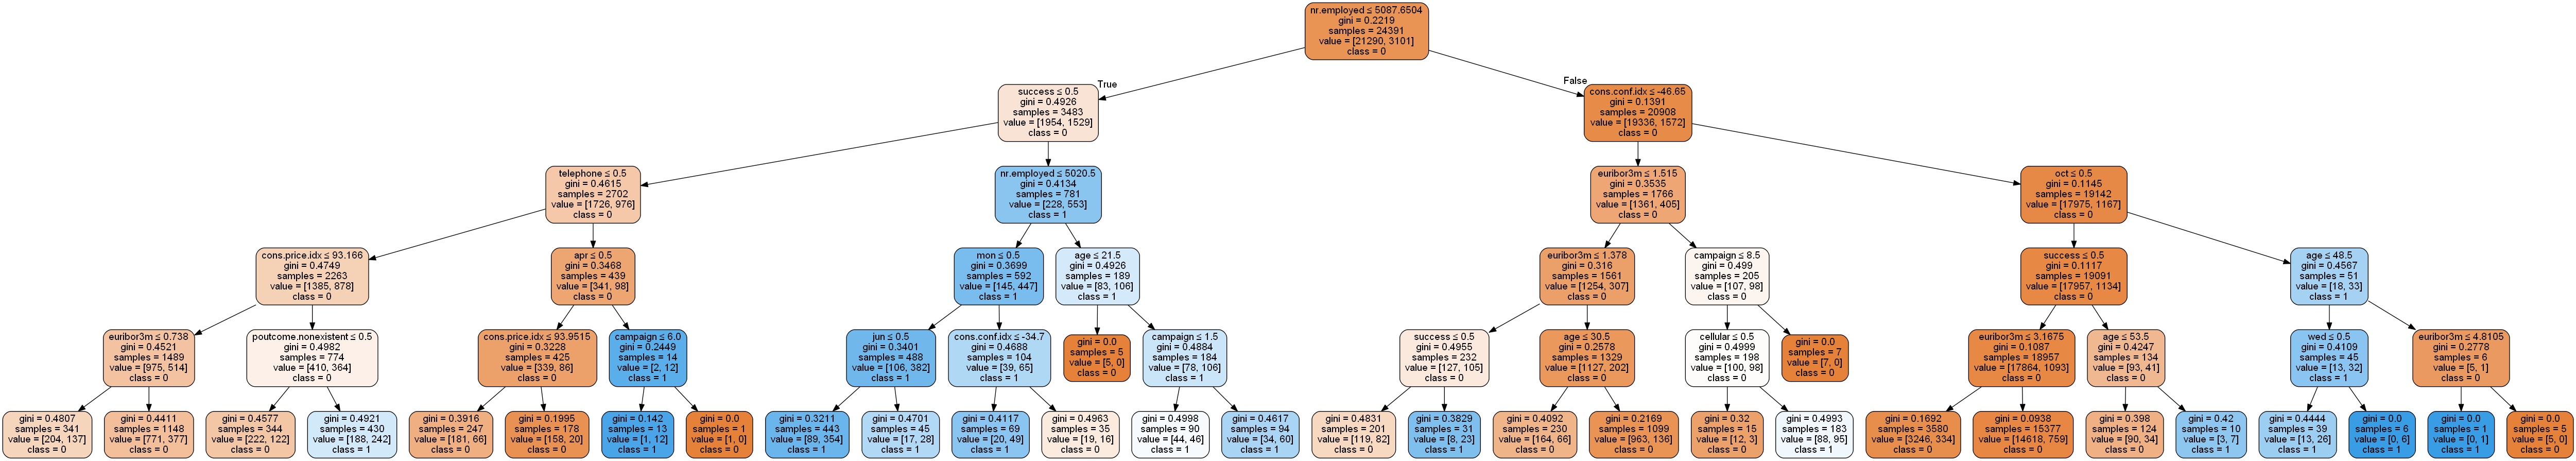
\includegraphics[width=4.5cm]{tree.png}\\
%  \caption{Single Decision Tree}\label{g05}
%\end{figure*}

%![plot](https://github.com/Johnzhong1468/MarketingCampaign/blob/master/tree.png)<br>
\subsection{random forest}

For our random forest model, we used 17 trees (by literature) in our forest. We set trees to grow to a maximum depth of 20 and assigned trees to randomly pick the square root of the total number of features to split upon. We will prune the trees later in the second half of the semester, to boost the prediction. The training and test accuracy are 0.9545 and 0.8759.

Random forest is not prone to overfitting since the majority vote prevents weighing heavily on single classification. Moreover, it prevents underfitting since trees are randomly assigned to a subset of features. The training and test accuracy are 0.9283 and  0.8992.

\begin{figure}[H]
  \centering
  % Requires \usepackage{graphicx}
  \includegraphics[width=6cm]{rf}\\
  \caption{prediction of random forest}\label{g10}
\end{figure}


\section{\color{blue}Summary of Results}
Going through the general procedure mentioned in previous part, we fit each model and estimate their performance. The critical part of results are listed below. To test the effectiveness, we calculated accuracy as the percentage of correctly classified customers. We found that logistic regression, the SVM and random forest are able to classify with an accuracy of 89.79\%, 89.42\% and 89.92\%, respectively (See {\color{red}Table \ref{T02}}). 

In a nutshell, the three models are of high accuracy, which implies they has relatively low bias. Note that the training-testing difference between random forest is higher than other models, which may imply that it has higher variance.

Logistic model is a traditional and prevalent model for classification. It can be estimated readily, especially when it is compared with SVM. The accuracy of considered models doesn't have significant difference. Thus, logistic model is more preferable while classifying and recognizing potential customers. Sometimes, may be the classic model hits the point.

\begin{table}[H]%[!htp]
  \centering
  \begin{tabular}{|l|c|c|l|}
     \hline
 Model   & \makecell[tl]{Training \\Accuracy} & \makecell[tl]{Testing\\ Accuracy} &Note\\ \hline
Lasso & 0.0210 &N.A. & Discarded\\ \hline
Ridge & 0.2116&0.1973&substandard\\ \hline
 Logistic & 0.9015 &  0.8979& generalized\\ \hline
 SVM & 0.8991 & 0.8942&generalized\\ \hline
\makecell[tl]{Decision Tree\\(depth=17)} &0.9545 &0.8759&-\\ \hline
Random Forest& 0.9284 & 0.8992&generalized\\ \hline
   \end{tabular}
  \caption{Preliminary Results}\label{T02}
\end{table}


\section{\color{blue}Conclusion}
By using techniques we learned in class such as cross validation, one-hot encoding,generalized low rank models, we can conduct our research fruitfully. 
We can assort lasso, ridge, logistic regression, svm and so on in a generalized framework. By choosing optimal loss function and regularizer, we can adapt the model to solve various real-world problems. Using proximal gradient descent and other iterate method, problems can be solved.

From the discussion above, we are able to classify the clients with great potential fairly well with 89\% accuracy. Just by analysing the previous contact with clients and the background information of them, entrepreneurs can easily focus on their target customers.

Since logistic regression is a linear model, it is not able to capture the inherit phenomena in the data set especially for continuous variables. With random forest, we were able to achieve an accuracy of 90\%. We are fairly confident that our model will be able to generalize to new client data because random forest is very flexible and can adjust itself since it takes samples of the features to split upon.





 \end{multicols}
\end{document}


